\documentclass{article}
\usepackage[UTF8]{ctex}
\usepackage{amsfonts}
\usepackage{amsmath}
\usepackage{float}
\usepackage{graphicx}
\usepackage{subcaption}
\usepackage{url}

\newcommand{\Bezier}{B\'ezier}%Bézier

\usepackage{color}

% paragraph
\setlength{\parindent}{0pt}
\setlength\parskip{\baselineskip}
\renewcommand{\baselinestretch}{1.2}

\begin{document}
	
	% 标题
	\title{《计算机辅助几何设计》作业}
	\author{ID号: 048  \qquad  姓名: 郑涛}  %递交作业时填上ID号和姓名
	\date{2024年11月16日}
	\maketitle
	1. Program and draw a perspective projection of a cube with center x and side length 2d on
	a 2D plane, where point x and the value of d are specified by the user. Make reasonable
	assumptions about camera parameters and orientation.
	
	我选的相机位置为(0,0,0),平面为垂直于z轴,朝向立方体的方向,平面的z坐标也作为输入参数。
	\section*{结果}
	\begin{figure}[H]
		\centering
		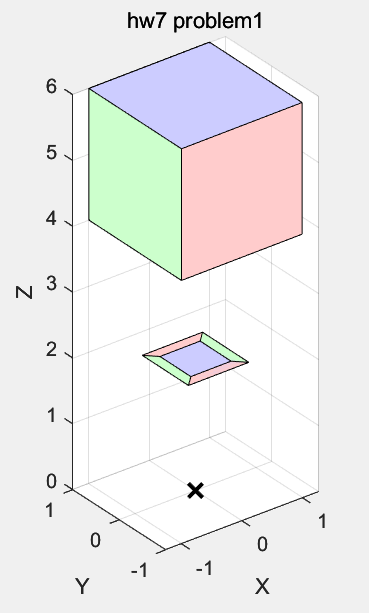
\includegraphics[scale=0.5]{7_1}
		\label{fig:71}
	\end{figure}
	
	
	2. Draw an ellipse $\frac{x^2}{a^2}+\frac{y^2}{b^2}=1$ and a hyperbola $\frac{x^2}{a^2}-\frac{y^2}{b^2}=1$ using rational
	quadratic B´ezier splines, with as few segments as possible. Parameters a and b are
	specified by the user.
	
	3. In 3D space, draw the B´ezier curves from the previous problem represented in homogeneous coordinates (i.e., the three-dimensional curves before projection transformation).
	
	\section*{实验思路}
	根据课上推导,二次有理Bezier曲线可以表示为:
	$$B(t)=\frac{(1-t)^2P_0+2t(1-t)wP_1+t^2P_2}{(1-t)^2+2t(1-t)w+t^2}$$
	根据平移不变性,不妨设$P_0=-P_2$,则有
	$$B(0.5)=\frac{wP_1}{w+1}$$
	\begin{figure}[H]
		\centering
		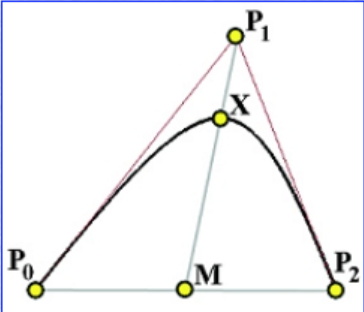
\includegraphics[scale=0.5]{idea}
		\label{fig:idea}
	\end{figure}
	设$P_0P_2$的中点为$M$,$P_1M$与有理Bezier曲线的交点为$X$,则有:
	$$\frac{MX}{MP_1}=\frac{w}{1+w}$$
	选定控制点后,根据上述公式求得$w$,然后带入求出曲线即可。
	取$-w$时即为共轭曲线
	\section*{结果}
	\subsection{ellipse}
	选取控制点为$P_0(a,0),P_1(a,b),P_2(0,b)$,求得$w=\frac{\sqrt{2}}{2}$。
	\begin{figure}[H]
		\centering
		\begin{minipage}{0.5\linewidth}
			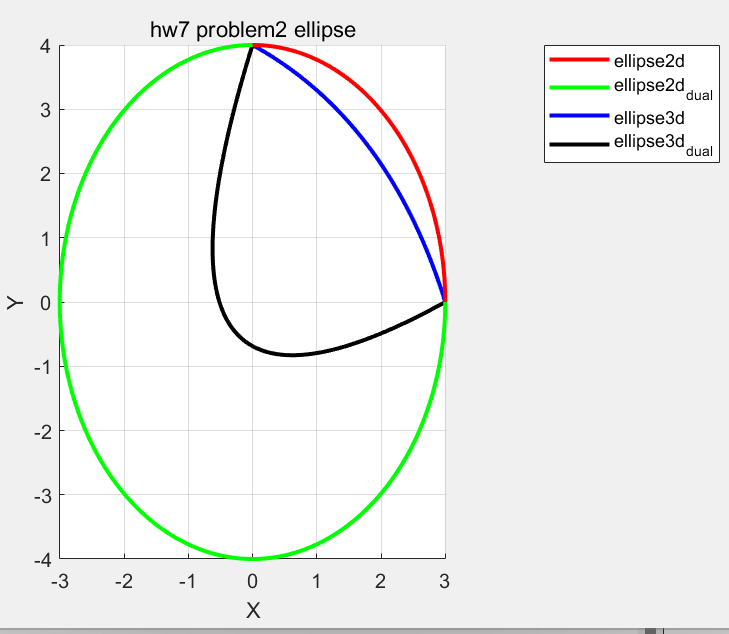
\includegraphics[scale=0.6]{7_2_ellipse2d}
			\label{fig:72ellipse2d}
		\end{minipage}
	\hfill
		\begin{minipage}{0.5\linewidth}
			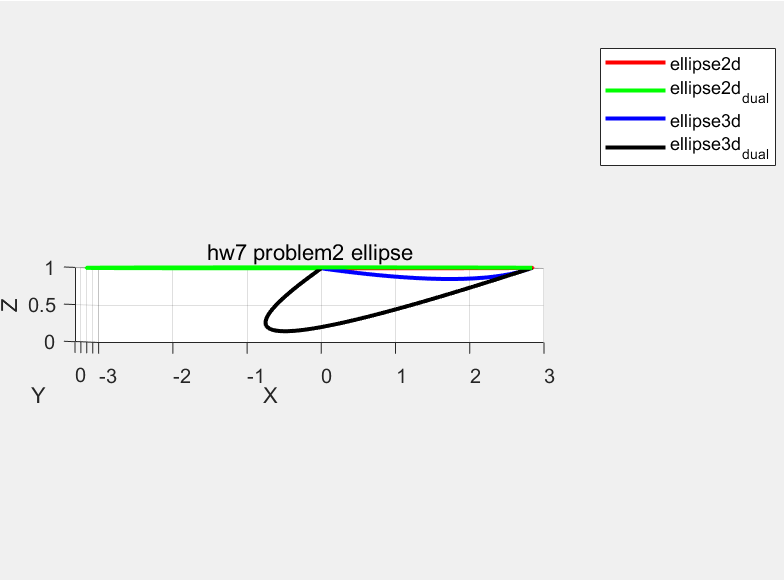
\includegraphics[scale=0.6]{7_2_ellipse3d}
			\label{fig:72ellipse3d}
		\end{minipage}
	\caption{ellipse,a=3,b=4}
	\label{ellipse}
	\end{figure}
	
	\subsection{hyperbola}
	选取控制点为$P_0(c,-\frac{b^2}{a}),P_1(\frac{a^2}{c},0),P_2(c,\frac{b^2}{a})$,求得$w=e=\frac{c}{a}$。
	\begin{figure}[H]
		\centering
		\begin{minipage}{0.5\linewidth}
			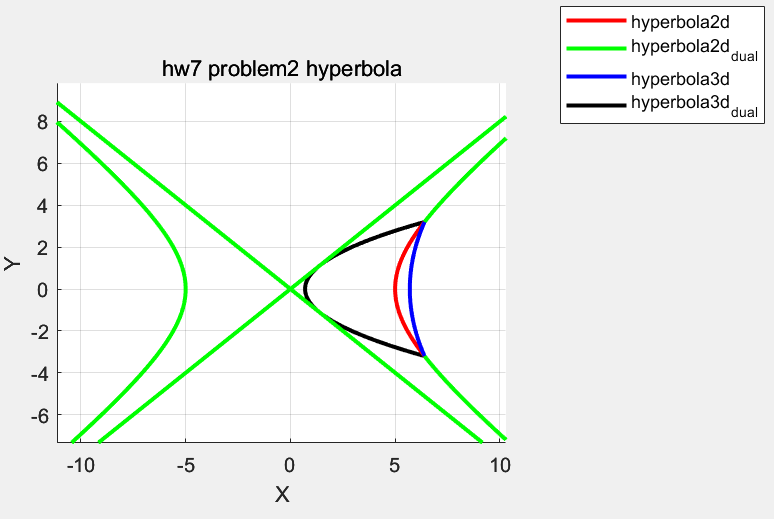
\includegraphics[scale=0.6]{7_2_hyperbola2d}
			\label{fig:72hyperbola2d}
		\end{minipage}
		\hfill
		\begin{minipage}{0.5\linewidth}
			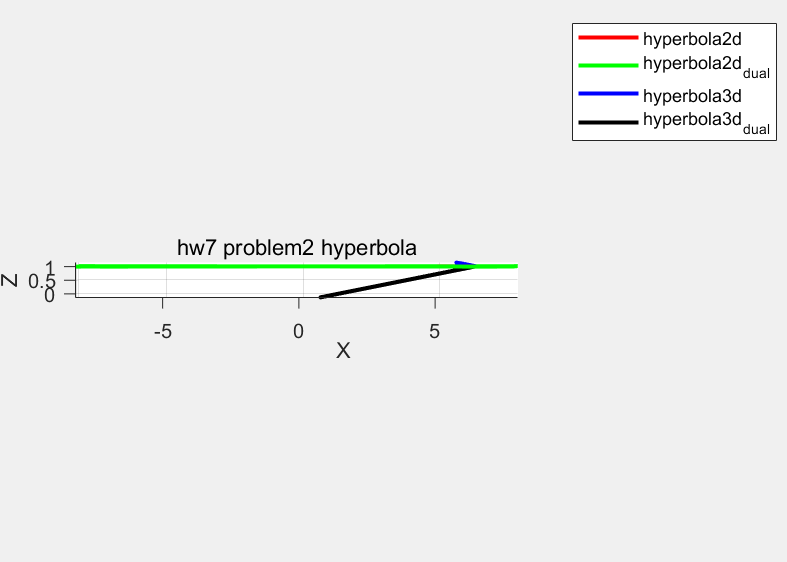
\includegraphics[scale=0.6]{7_2_hyperbola3d}
			\label{fig:72hyperbola3d}
		\end{minipage}
		\caption{hyperbola,a=5,b=4}
		\label{ellipse}
	\end{figure}
\end{document}











